\documentclass[12pt, oneside, a4paper]{ctexart}
\usepackage{amsmath}
\usepackage{amssymb}
\usepackage{caption}
\usepackage{ctex}
\usepackage{enumerate}
\usepackage{float}
\usepackage[{top=2.54cm, bottom=2.54cm, left=3.18cm, right=3.18cm}]{geometry}
\usepackage{graphicx}
\usepackage[breaklinks, colorlinks=false, hidelinks]{hyperref}
\usepackage{longtable}
\usepackage{mathptmx}
\usepackage{multirow}
\usepackage{tabularx}
\usepackage{xcolor}
\usepackage{xeCJK}

\ctexset{
    section={
        name={,、},
        number={\chinese{section}},
        format=\heiti\raggedright\zihao{3}\bfseries,
        aftername={\hspace{0.5em}},
        beforeskip=1ex,
        afterskip=1ex,
    },
    subsection={
        name={,.},
        number={\arabic{subsection}},
        format=\songti\raggedright\zihao{-4}\bfseries,
        aftername={\hspace{0.5em}},
        beforeskip=0ex,
        afterskip=0ex,
    },
}
\newlength{\stepbodyindent}
\AtBeginDocument{\settowidth{\stepbodyindent}{{\songti\zihao{-4}\bfseries 1.\hspace{0.5em}}}}
\newcommand{\stepbody}[1]{%
    \par
    {\setlength{\leftskip}{\stepbodyindent}\setlength{\parindent}{0pt}#1\par}%
}
\pagestyle{plain}
\DeclareCaptionLabelFormat{figuretitle}{图#2}
\captionsetup[figure]{labelformat=figuretitle,labelsep=space,font=small}
\DeclareCaptionLabelFormat{tabletitle}{表#2}
\captionsetup[table]{labelformat=tabletitle,labelsep=space,font=small}
\setmainfont{Times New Roman}
\setCJKmainfont[AutoFakeBold={2}]{SimSun}
\setCJKfamilyfont{zh}{SimSun}
\setCJKfamilyfont{ja}{BIZ UDMincho}
\xeCJKDeclareCharClass{CJK}{
  "24EA,
  "2460->"2473,
  "3251->"32BF,
  "24FF,
  "2776->"277F,
  "24EB->"24F4
}


%----------分割线----------%


\begin{document}


\thispagestyle{empty}
\begin{center}{
    \fontsize{26pt}{26pt}\selectfont
    \vspace*{1.5\baselineskip}
    
\includegraphics[width=0.6\textwidth]{pics/tongji-university-logo-1024px.png}\\
    [\baselineskip]
    \heiti{轨道交通综合实验报告（二）}\\
    \vspace*{1\baselineskip}
    \fontsize{18pt}{24pt}\selectfont
    \songti{
        \begin{tabular}{l}
            {\heiti{}实验日期：}2026年10月15日      \\
            {\heiti{}实验名称：}车辆平稳性测试实验        \\
            {\heiti{}实验人员：}肖哲夫~~2352670     \\
            \qquad\qquad\quad{}蒙卫焓~~2352250 \\
            \qquad\qquad\quad{}梁耀钦~~2352398 \\
            \qquad\qquad\quad{}李海炳~~2353848 \\
            {\heiti{}实验地点：}轨道交通试验线
        \end{tabular}
    }
    }
\end{center}
\newpage{}
\setcounter{page}{1}

\section{\heiti{实验目的}}
\par{}
测量地铁车辆运行时的垂向和横向加速度，计算Sperling平稳性指标，并评价车辆的运行平稳性。


\section{\heiti{实验设备}}
\par{}
YD615D型加速度传感器2个、USB6008型数据采集卡1张、TL-1型信号调理器、安装有LabVIEW软件的计算机1台。

\section{\heiti{实验步骤}}
\subsection{\heiti{测试设备安装及调试}}
\stepbody{安装并调试测试设备，检查仪器和采集程序，准备车上使用的220~V交流电源。}
\subsection{\heiti{车体加速度测点布置}}
\stepbody{根据指导书引用的GB5599-85规定，在距车体Ⅰ、Ⅱ位心盘一侧1000~mm的车体地板面上布置加速度传感器，测量横向和垂向加速度。测点布置如图1所示，本次实验的测点选在$\mathrm{S_{12}}$处；测试系统的实物接线如图2所示。}
\begin{figure}[htbp]
    \centering
    \vspace{-0.1cm}
    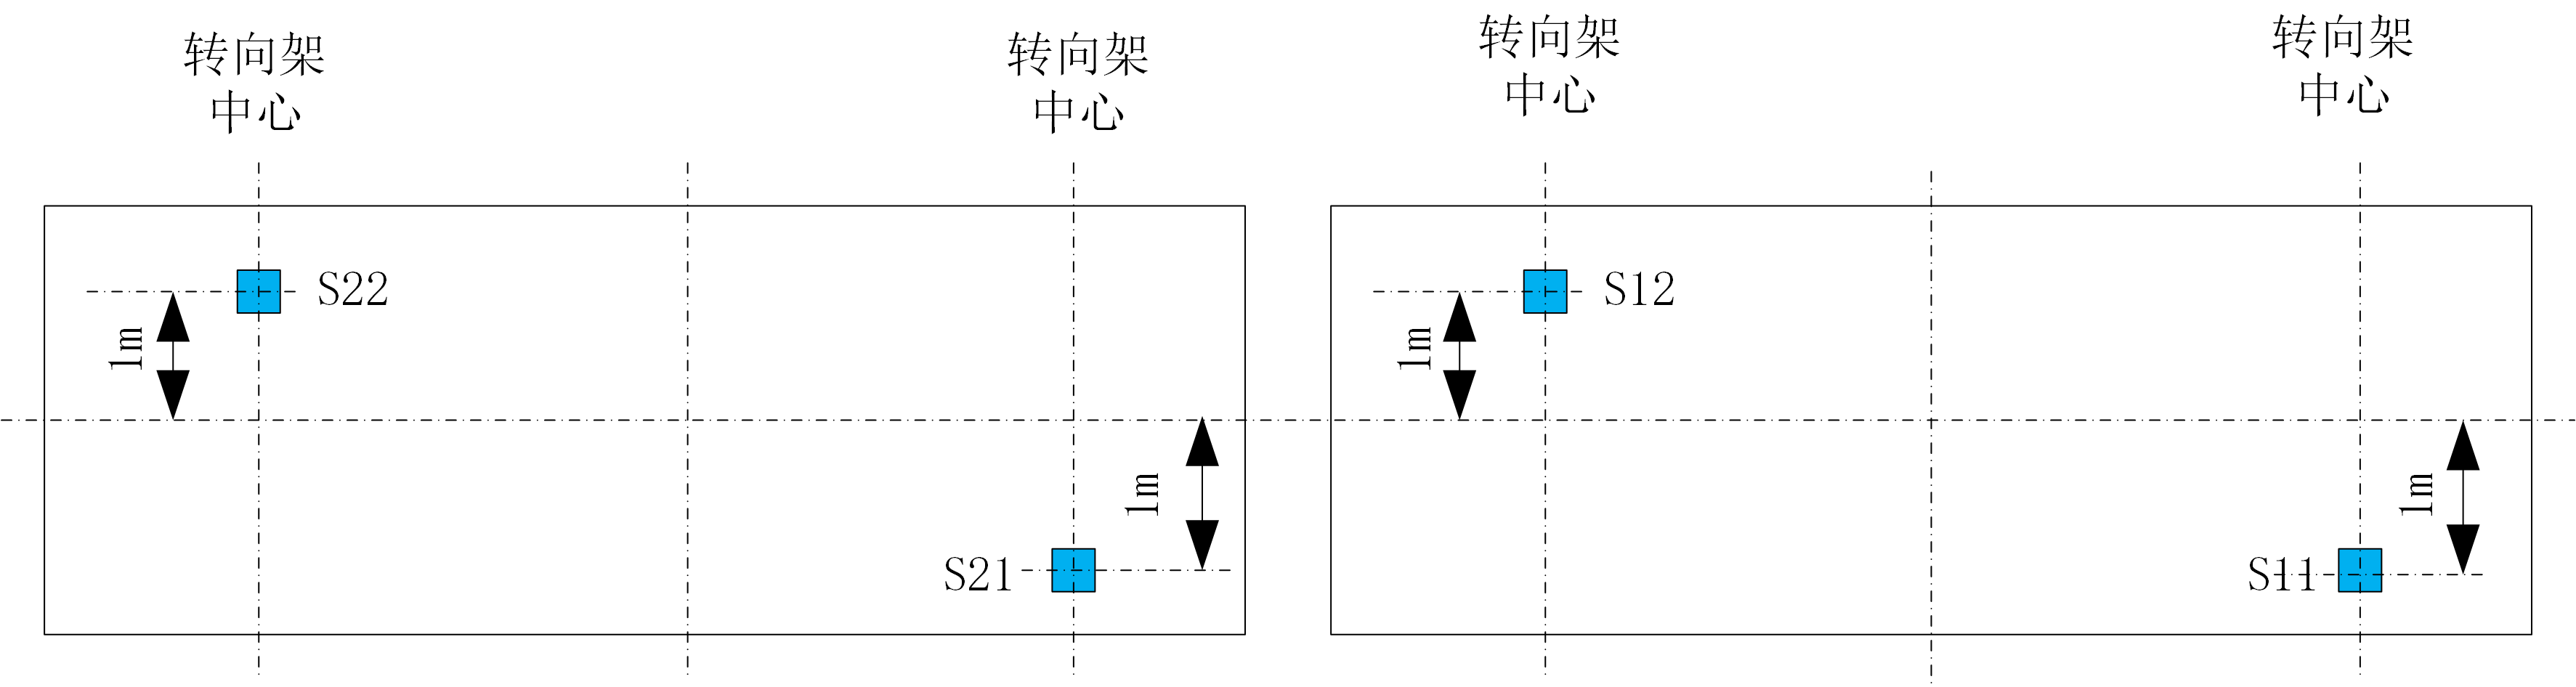
\includegraphics[width=0.98\textwidth]{pics/01.png}
    \vspace{-0.1cm}
    \caption{加速度测量点布置}
    \vspace{-0.5cm}
\end{figure}
\begin{figure}[htbp]
    \centering
    \begin{minipage}[t]{0.48\textwidth}
        \centering
        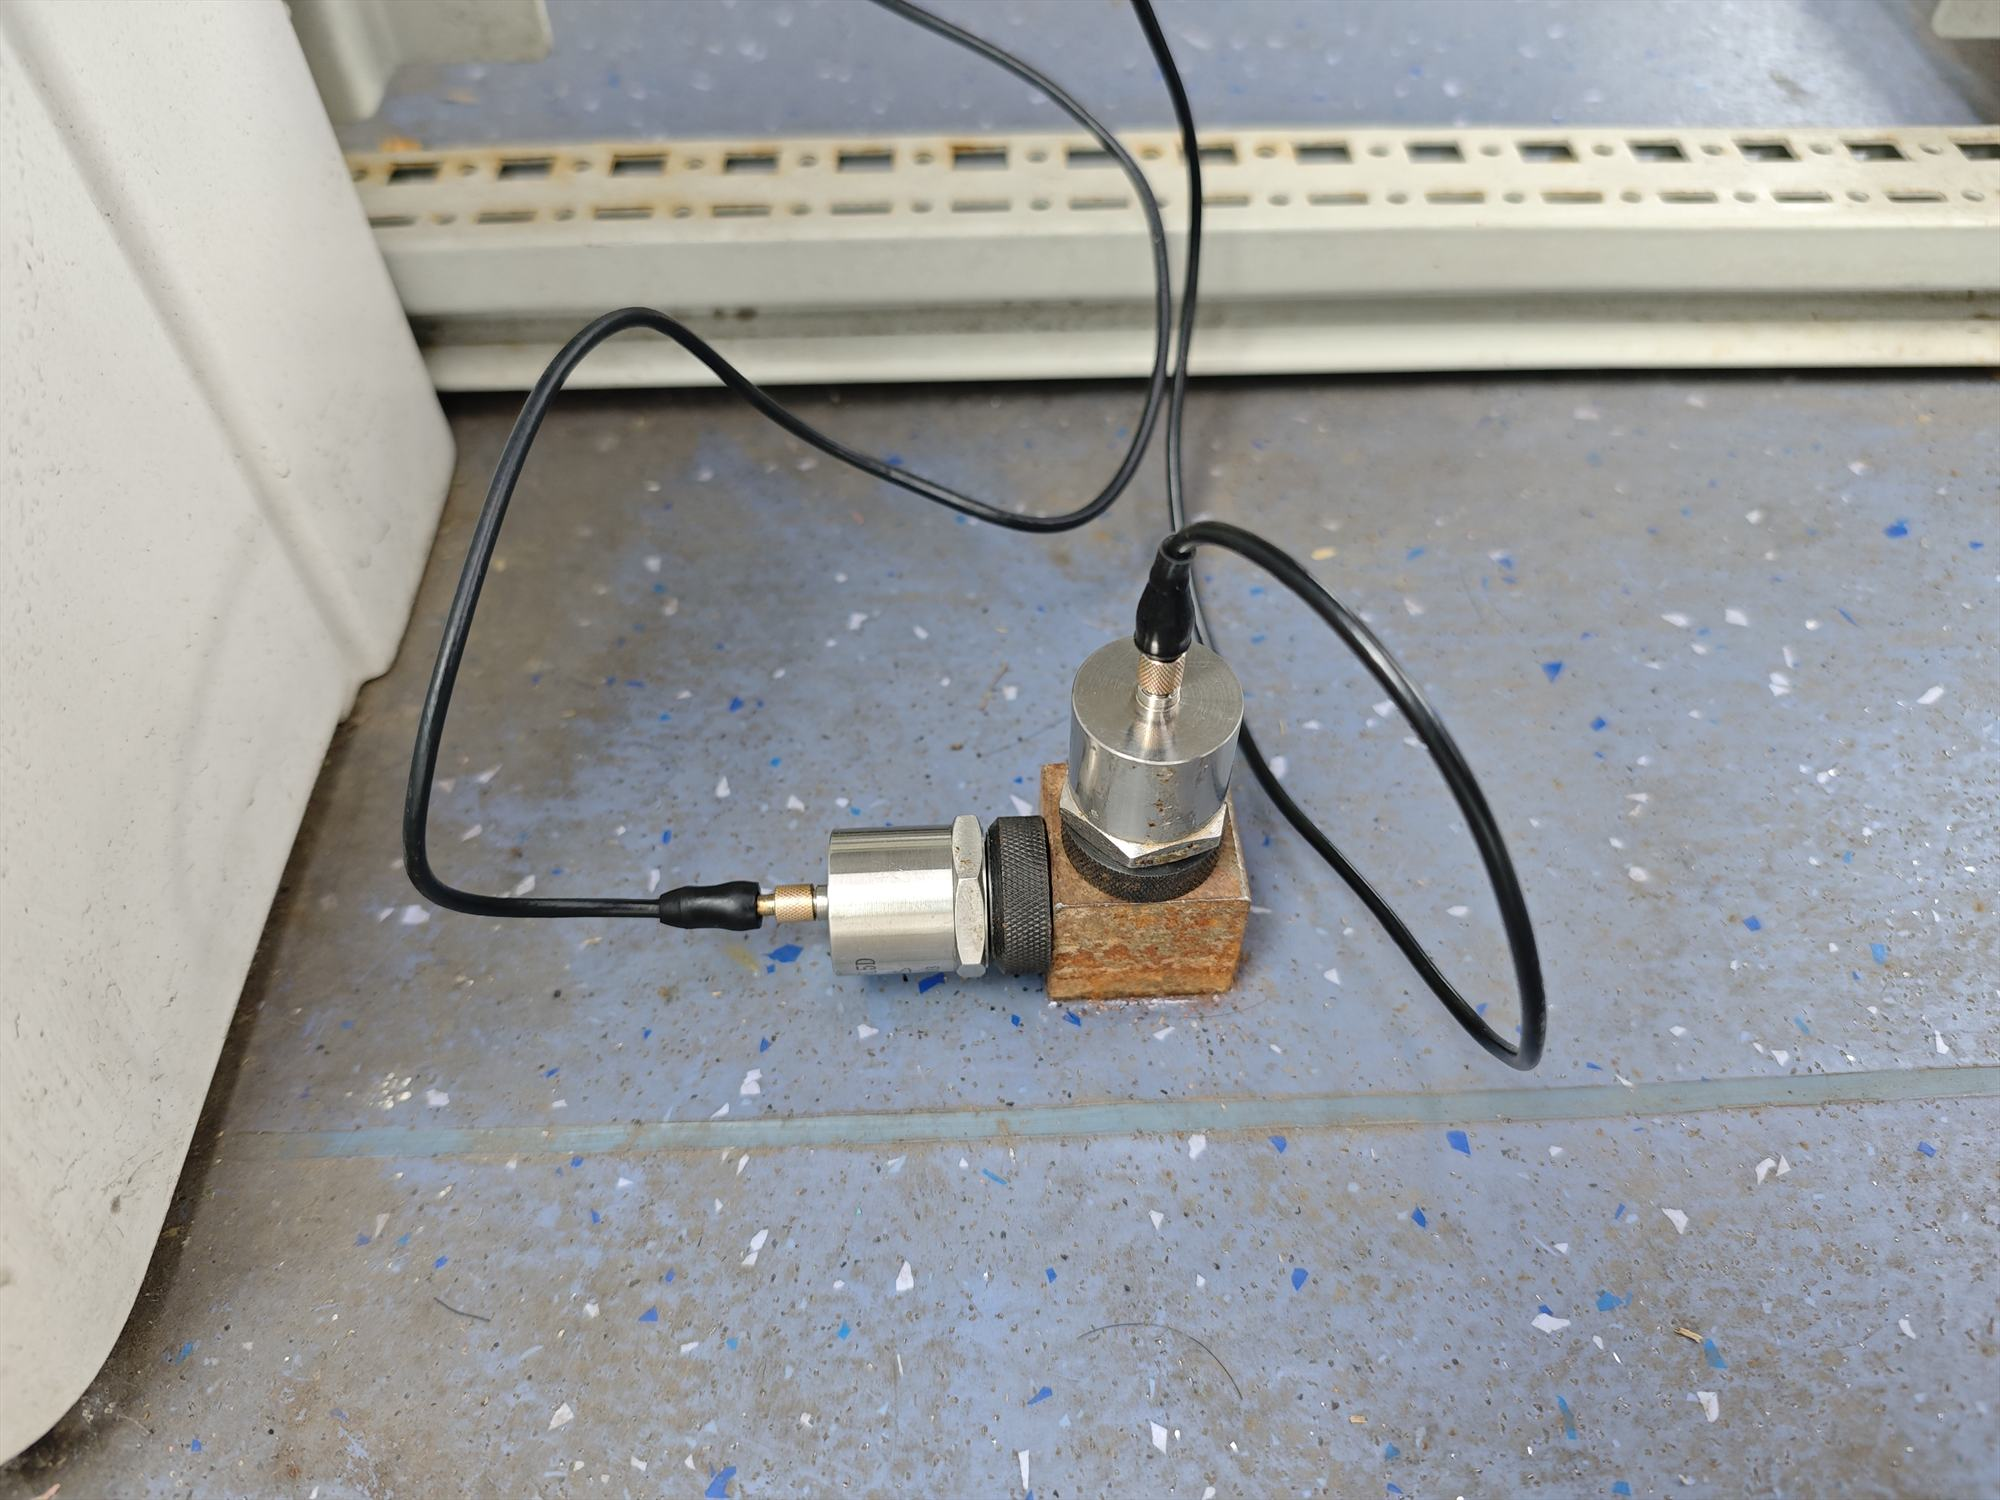
\includegraphics[width=\linewidth]{pics/02a.jpg}
    \end{minipage}\hfill
    \begin{minipage}[t]{0.48\textwidth}
        \centering
        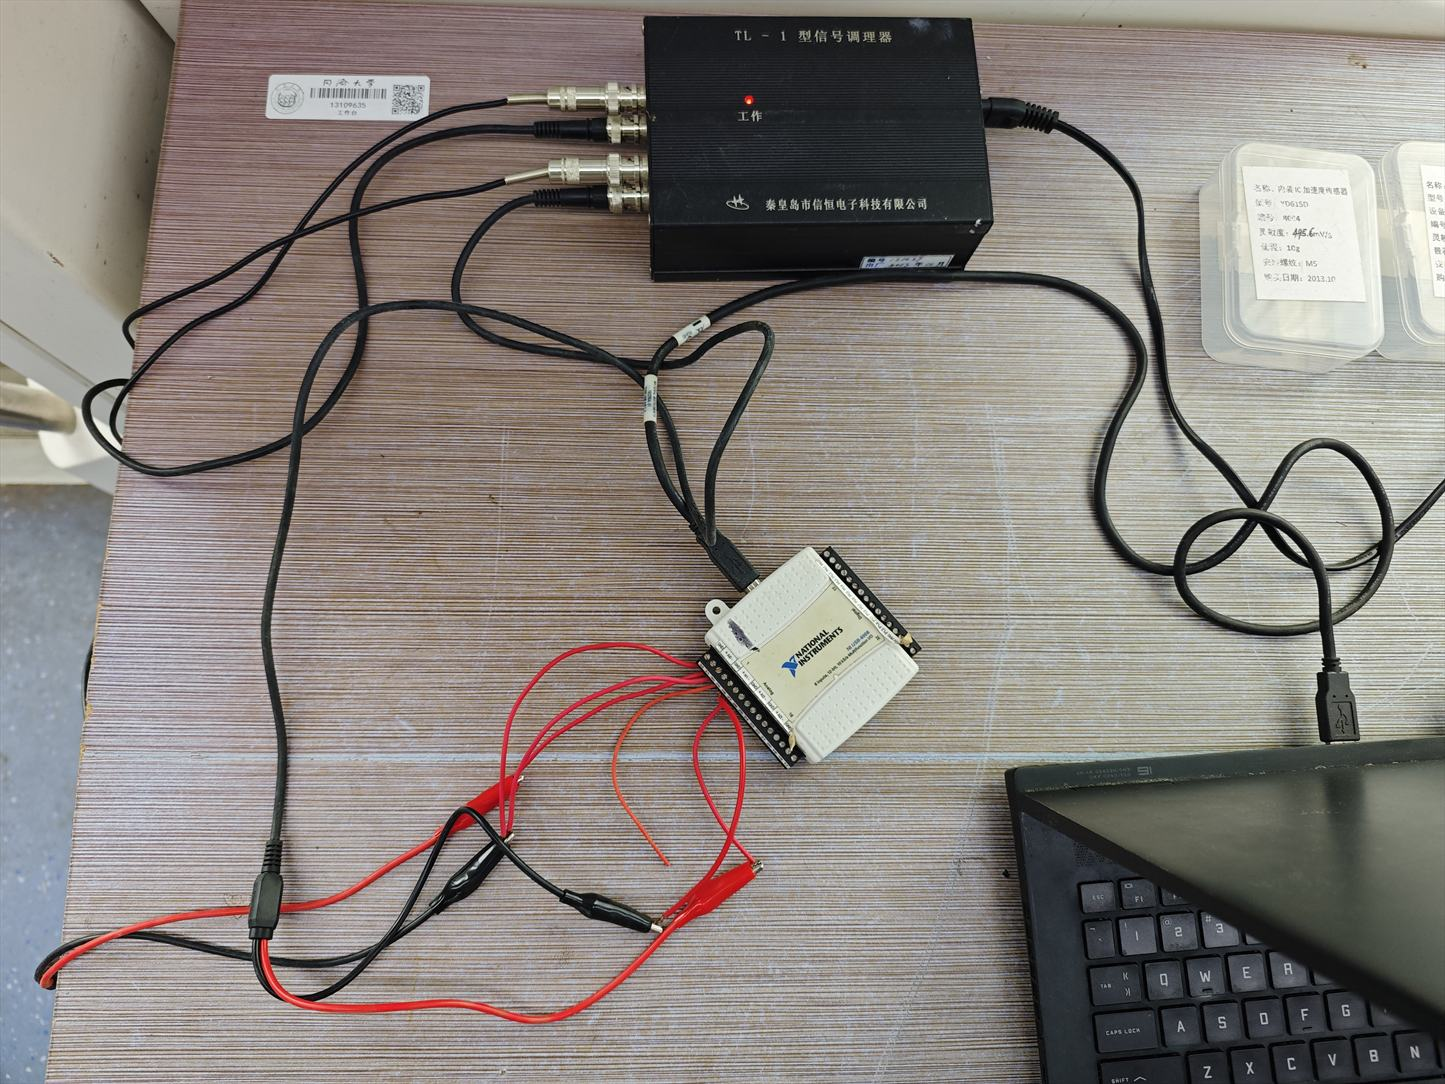
\includegraphics[width=\linewidth]{pics/02b.jpg}
    \end{minipage}
    \caption{测试系统实物接线}
    \vspace{-0.5cm}
\end{figure}
\subsection{\heiti{数据采集}}
\stepbody{在直线区段记录速度稳定时的车体垂向、横向加速度，采样频率设为256~Hz。}
\subsection{\heiti{线路测试}}
\stepbody{在嘉定校区轨道交通试验线上采用人工驾驶，运行速度分别取30、40~km/h。由于实验条件限制，本次实验在30~km/h工况下完成6次单程测试（往返3次），获得6组数据；在40~km/h工况下完成3次单程测试，获得3组数据。}
\subsection{\heiti{数据处理}}
\stepbody{本次数据处理以5~s为一个数据段，计算各速度等级下的垂向、横向Sperling平稳性指标；分段依据及具体处理方法见后文。}
\subsection{\heiti{测试设备拆卸}}
\stepbody{线路测试结束后，拆卸测试设备。}

\section{实验报告}
\subsection{\heiti{加速度传感器的使用方法}}
\par{}
将两只加速度传感器通过磁性底座固定于测点，使其敏感轴分别沿垂向和横向布置，并连接相应信号线。
\par{}
随后，将两根信号线另一端的BNC接头分别接入信号调理器对应通道的输入端，再将各通道的输出端接入数据采集卡。其中，信号调理器通道1的输出端连接数据采集卡的端口2、3，通道2的输出端连接端口5、6，最后通过USB线将数据采集卡接入计算机。
\par{}
最终连接结果如图2所示。

\subsection{\heiti{测试系统的标定系数}}
\begin{figure}[htbp]
    \centering
    \vspace{-0.1cm}
    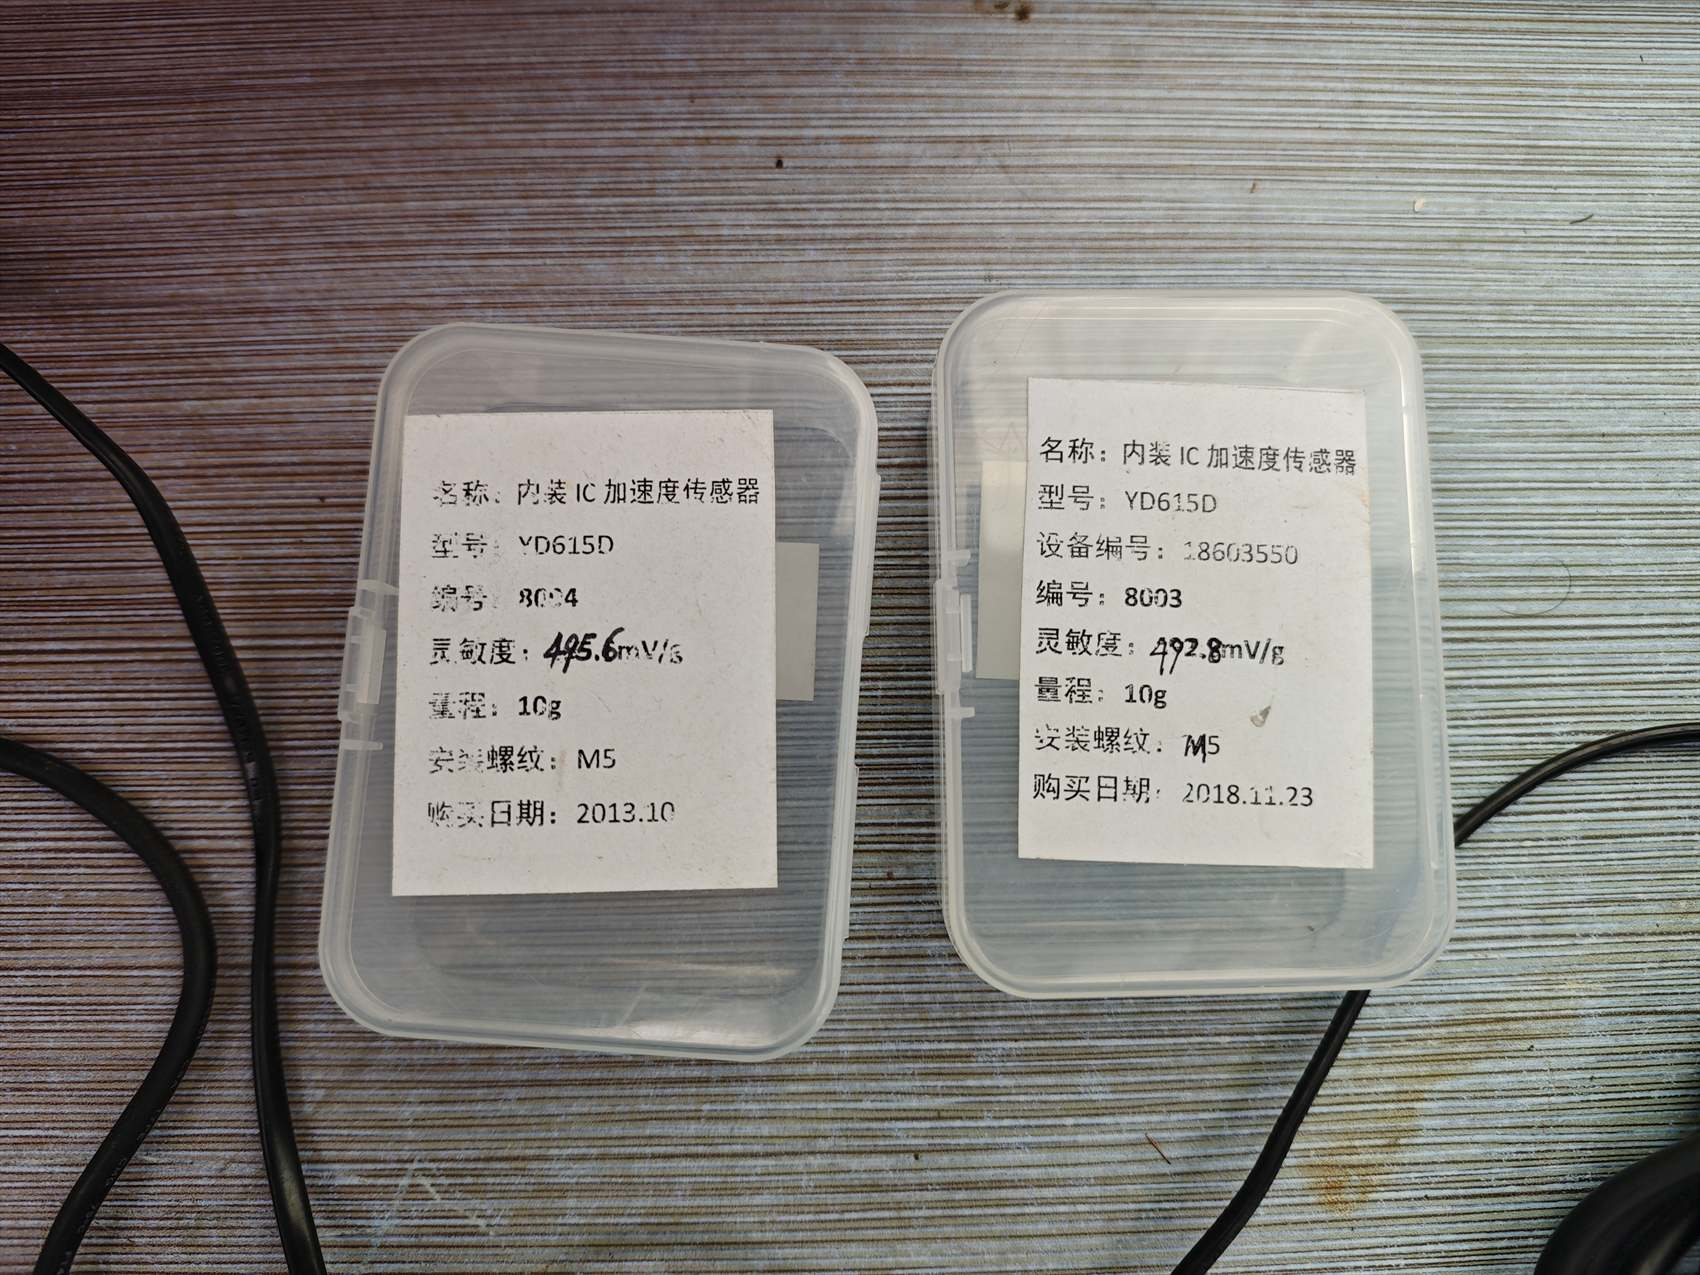
\includegraphics[width=0.7\textwidth]{pics/03.jpg}
    \vspace{-0.1cm}
    \caption{加速度传感器技术参数}
    \label{fig:sensor-parameters}
    \vspace{-0.5cm}
\end{figure}
\par{}
传感器的技术参数如图\ref{fig:sensor-parameters}所示，其中垂向、横向加速度传感器的灵敏度分别为495.6~mV/$g$与492.8~mV/$g$。设传感器灵敏度为$S$，信号调理器的电压增益为$G$，则加速度与采集电压的关系为
\begin{equation*}
    a(t)=K_a\Delta u(t),\qquad K_a=\frac{1000}{GS}.
\end{equation*}
\par{}
式中，$\Delta u(t)$为采集电压相对于零加速度基准电压的变化量，单位为V；$S$以mV/$g$计，$G$为无量纲电压增益，$K_a$的单位为$g$/V。按$G=1$计算，垂向和横向的$K_a$分别约为2.01776~$g$/V与2.02922~$g$/V。将电压变化量乘以对应换算系数，即可得到以$g$为单位的加速度。

\subsection{\heiti{实验加速度时域波形}}
\par{}
9次测试的加速度时域波形如图\ref{fig:time-waveforms}所示。垂向加速度幅值总体大于横向加速度幅值，与实验过程中的主观感受基本一致。
\begin{figure}[htbp]
    \centering
    \vspace{-0.3cm}
    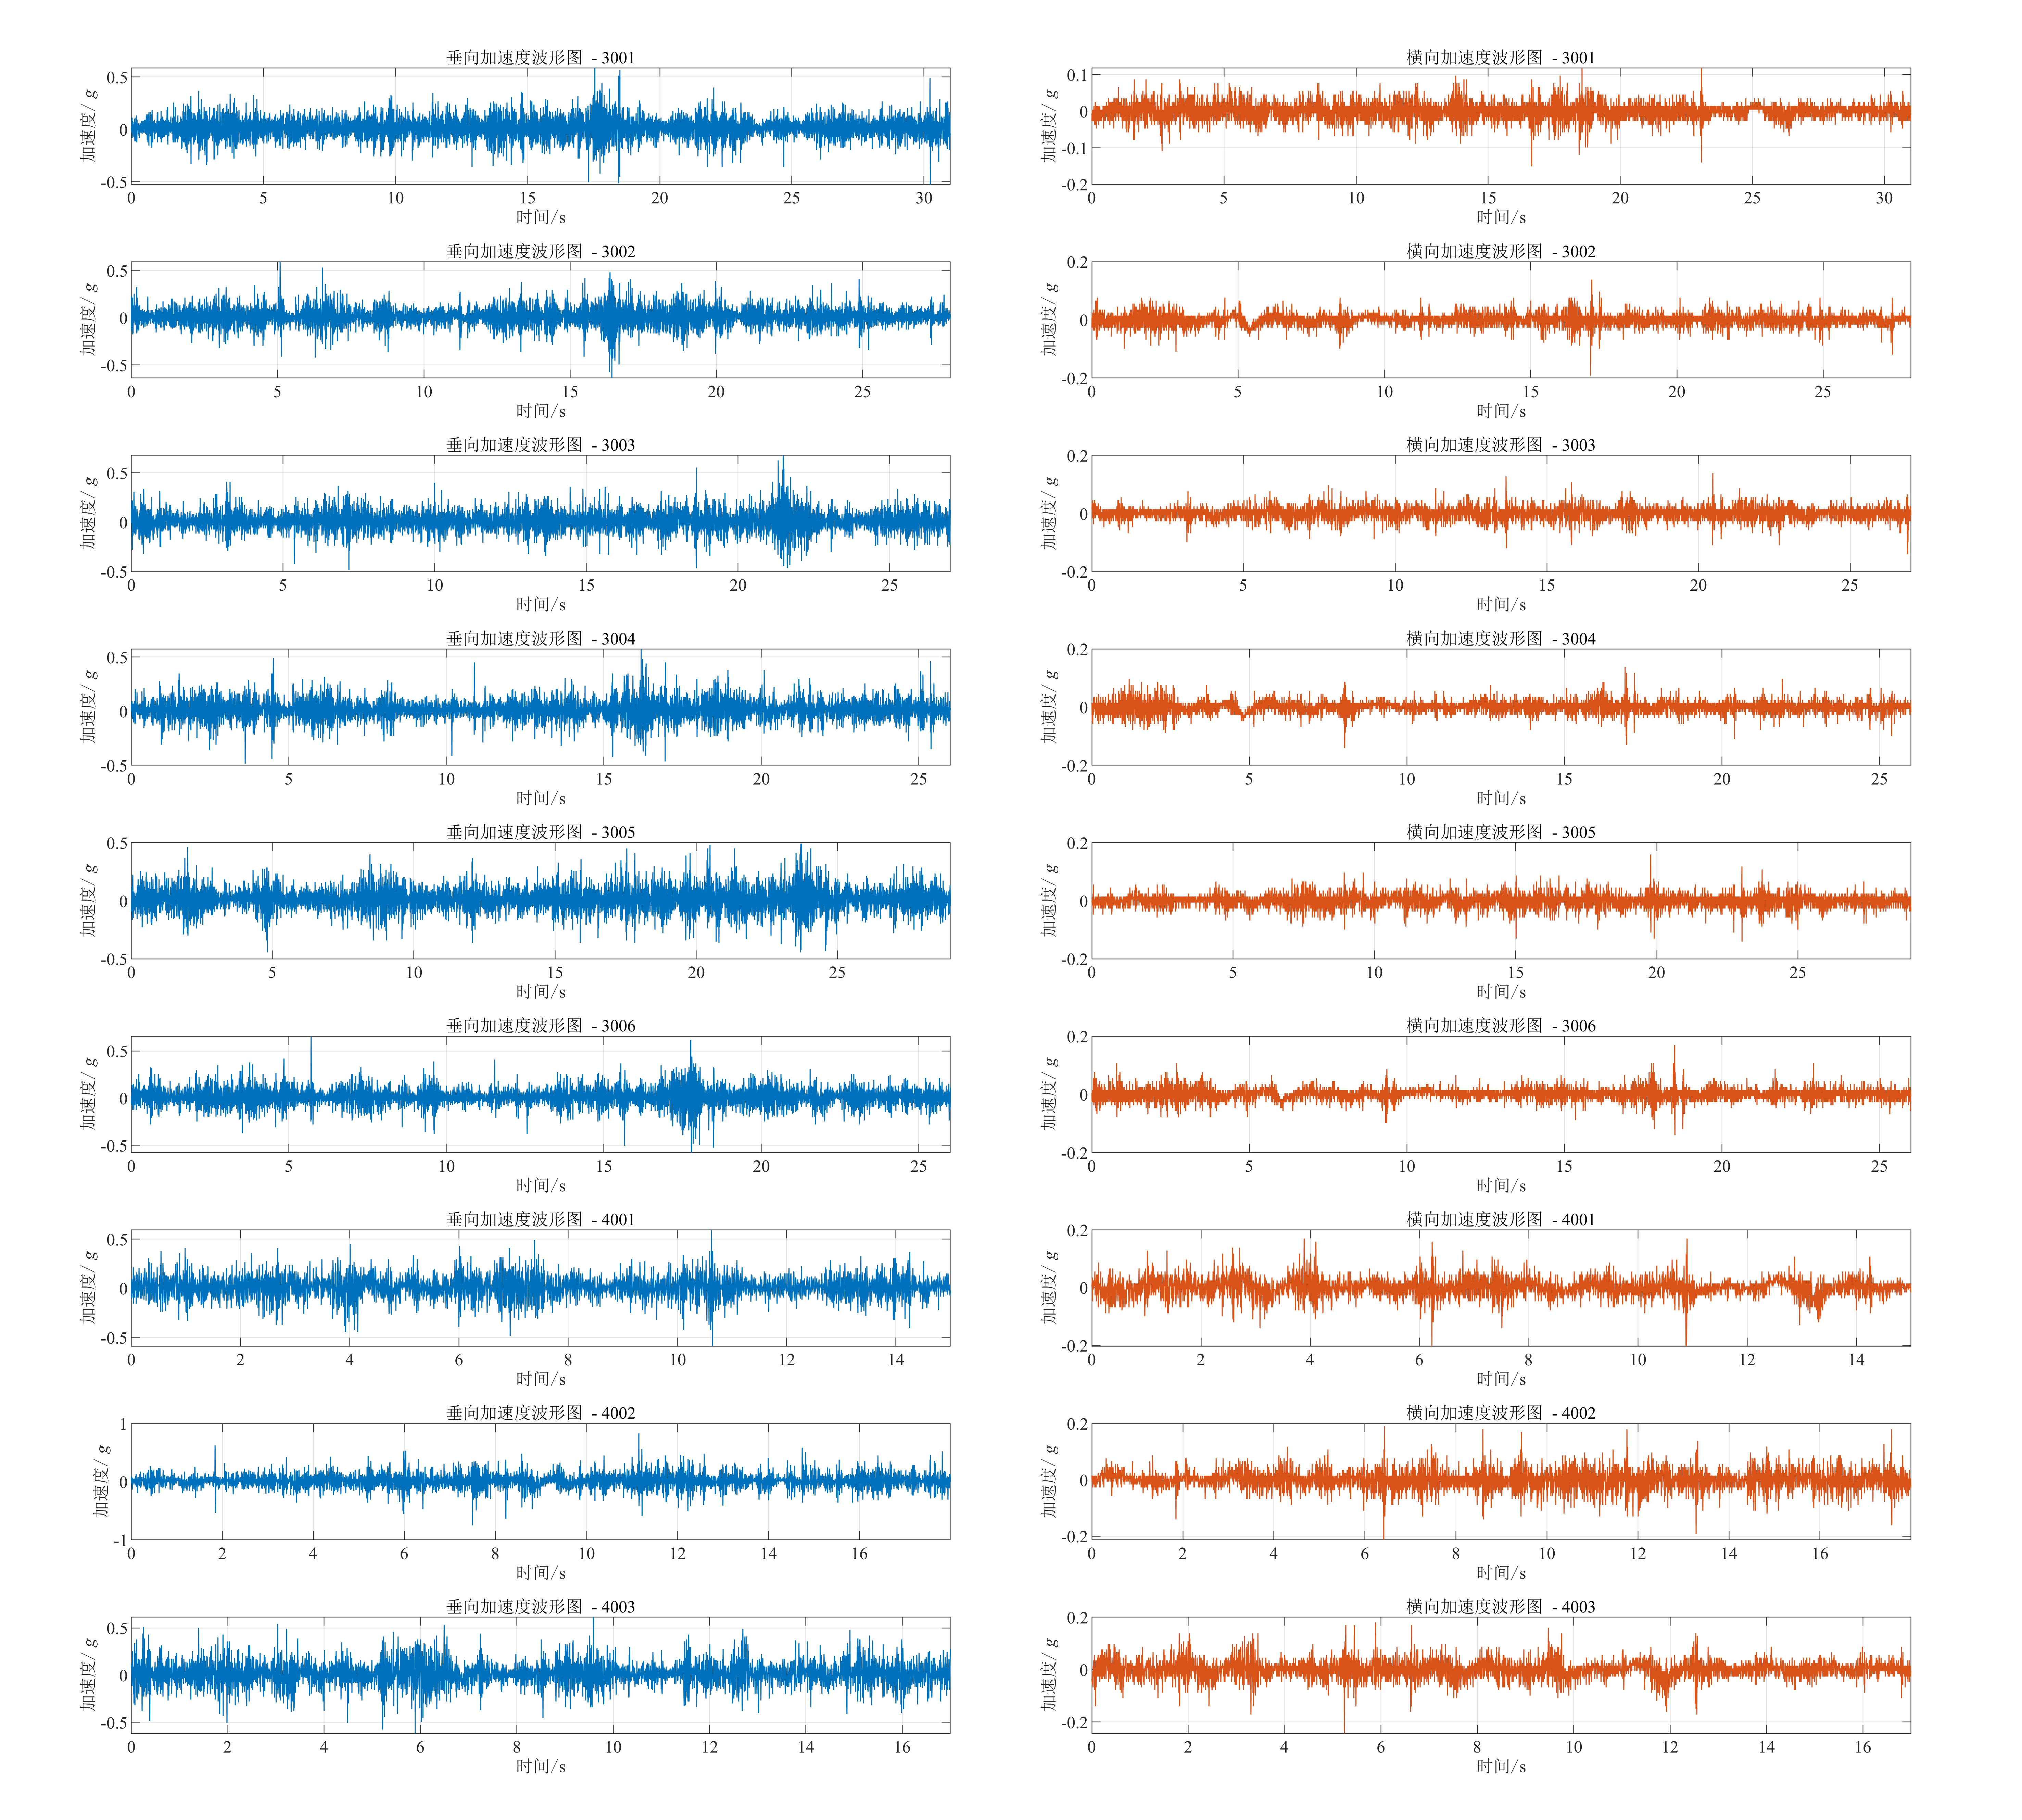
\includegraphics[trim=18mm 0mm 25mm 0mm,clip,width=0.98\linewidth]{pics/99_all_time_waveforms.png}
    \vspace{-0.5cm}
    \caption{九次测试加速度时域波形}
    \label{fig:time-waveforms}
    \vspace{-0.5cm}
\end{figure}
\par{}

\subsection{\heiti{数据处理结果与车辆平稳性分析}}
\par{}
本次实验使用课程提供的Sperling指标实时计算程序，通过录屏记录其输出的平稳性指标；同时针对记录的时域数据，另写一份MATLAB脚本以计算Sperling指标，并对比两种方法的计算结果。实时计算结果如表\ref{tab:realtime-sperling}所示。数据组编号前两位表示运行速度，后两位表示该速度下的测试序号。表中$W_j$表示该组数据按时间顺序记录的第$j$个数据段的平稳性指标，$\mbox{-{}-}$表示无对应数据，$\overline{W}$为该组同一方向有效指标的算术平均值。
\newpage{}
\begingroup
\small
\renewcommand{\arraystretch}{1.3}
\setlength{\tabcolsep}{3pt}
\begin{center}
    \vspace{-0.2cm}
    \captionof{table}{实时记录的平稳性指标}
    \label{tab:realtime-sperling}
    \begin{tabularx}{\linewidth}{|c|*{8}{>{\centering\arraybackslash}X|}}
        \hline
        数据组                   & 方向 & $W_1$   & $W_2$   & $W_3$   & $W_4$       & $W_5$       & $W_6$       & $\overline{W}$ \\
        \hline
        \multirow{2}{*}{3001} & 垂向 & 2.11584 & 2.12107 & 2.10418 & 2.21762     & 2.12864     & 1.99743     & 2.11413        \\
        \cline{2-9}
                              & 横向 & 1.54681 & 1.63856 & 1.67823 & 1.49266     & 1.67103     & 1.57298     & 1.60005        \\
        \hline
        \multirow{2}{*}{3002} & 垂向 & 2.30113 & 2.22837 & 2.08552 & 2.18482     & 2.22315     & \mbox{-{}-} & 2.20460        \\
        \cline{2-9}
                              & 横向 & 1.53349 & 1.62607 & 1.66048 & 1.49457     & 1.51694     & \mbox{-{}-} & 1.56631        \\
        \hline
        \multirow{2}{*}{3003} & 垂向 & 2.25958 & 2.10499 & 2.22190 & 2.11949     & 2.33191     & \mbox{-{}-} & 2.20757        \\
        \cline{2-9}
                              & 横向 & 1.54132 & 1.69179 & 1.71815 & 1.73104     & 1.56678     & \mbox{-{}-} & 1.64982        \\
        \hline
        \multirow{2}{*}{3004} & 垂向 & 2.26740 & 2.40145 & 1.97031 & 2.18099     & 2.20191     & \mbox{-{}-} & 2.20441        \\
        \cline{2-9}
                              & 横向 & 1.56926 & 1.77130 & 1.53770 & 1.45476     & 1.55485     & \mbox{-{}-} & 1.57757        \\
        \hline
        \multirow{2}{*}{3005} & 垂向 & 2.19465 & 2.08171 & 2.05568 & 2.12240     & 2.41810     & \mbox{-{}-} & 2.17451        \\
        \cline{2-9}
                              & 横向 & 1.50172 & 1.56546 & 1.62299 & 1.61198     & 1.48095     & \mbox{-{}-} & 1.55662        \\
        \hline
        \multirow{2}{*}{3006} & 垂向 & 2.27674 & 2.26200 & 2.13918 & 2.17353     & 2.36861     & \mbox{-{}-} & 2.24401        \\
        \cline{2-9}
                              & 横向 & 1.59224 & 1.59120 & 1.67272 & 1.45120     & 1.57988     & \mbox{-{}-} & 1.57745        \\
        \hline
        \multirow{2}{*}{4001} & 垂向 & 2.29706 & 2.29393 & 2.42466 & \mbox{-{}-} & \mbox{-{}-} & \mbox{-{}-} & 2.33855        \\
        \cline{2-9}
                              & 横向 & 1.96309 & 2.01739 & 1.86818 & \mbox{-{}-} & \mbox{-{}-} & \mbox{-{}-} & 1.94955        \\
        \hline
        \multirow{2}{*}{4002} & 垂向 & 2.26085 & 2.27133 & 2.56042 & \mbox{-{}-} & \mbox{-{}-} & \mbox{-{}-} & 2.36420        \\
        \cline{2-9}
                              & 横向 & 1.73764 & 1.77137 & 1.69348 & \mbox{-{}-} & \mbox{-{}-} & \mbox{-{}-} & 1.73416        \\
        \hline
        \multirow{2}{*}{4003} & 垂向 & 2.25983 & 2.34879 & 2.53259 & \mbox{-{}-} & \mbox{-{}-} & \mbox{-{}-} & 2.38040        \\
        \cline{2-9}
                              & 横向 & 1.95033 & 2.00668 & 1.85600 & \mbox{-{}-} & \mbox{-{}-} & \mbox{-{}-} & 1.93767        \\
        \hline
    \end{tabularx}
\end{center}
\endgroup
\par{}
后处理脚本的计算方法如下。
\par{}
由指导书和参考文件得，加速度以$g$为单位时，Sperling平稳性指标计算公式为
\begin{equation*}
    W=7.08\sqrt[10]{\frac{A^3}{f}F(f)}.
\end{equation*}
其中，$W$为无量纲平稳性指标，$A$为单一频率分量的加速度幅值（单位为$g$），$f$为该分量的频率（单位为Hz），$F(f)$为频率修正系数。
\par{}
该脚本将9组加速度数据按5~s连续、不重叠地分段，舍弃各组记录末尾不足5~s的部分。对每段数据去除均值后施加周期汉宁窗，再进行FFT，并补偿窗函数的相干增益，得到单边幅值谱，并选取0.5-40~Hz范围内的频率分量计算平稳性指标。
\par{}
参照课堂上提供的相关标准，垂向和横向分别采用频率修正系数$F_z(f)$和$F_y(f)$：
\begin{equation*}
    F_z(f)=
    \begin{cases}
        0.325f^2, & 0.5\leq f<5.9,  \\
        400/f^2,  & 5.9\leq f<20,   \\
        1,        & 20\leq f\leq40,
    \end{cases}
    \qquad
    F_y(f)=
    \begin{cases}
        0.8f^2,  & 0.5\leq f<5.4,  \\
        650/f^2, & 5.4\leq f<26,   \\
        1,       & 26\leq f\leq40.
    \end{cases}
\end{equation*}
\par{}
对于包含多个频率分量的加速度信号，将各频率分量对应平稳性指标的十次方求和，再开十次方根，得到该数据段的综合平稳性指标：
\begin{equation*}
    W=\sqrt[10]{\sum_{k\in\mathcal{K}}W_k^{10}}
    =7.08\sqrt[10]{
        \sum_{k\in\mathcal{K}}
        \frac{A_k^3}{f_k}F(f_k)
    }.
\end{equation*}
式中，$\mathcal{K}$为计算频带内的频率点集合，$A_k$为单边幅值谱中对应频率$f_k$的加速度幅值（单位为$g$），$W_k$为该频率分量对应的平稳性指标。垂向和横向分别代入对应的频率修正系数，计算各5~s数据段的平稳性指标，结果见表\ref{tab:postprocessed-sperling}。
\begingroup
\small
\renewcommand{\arraystretch}{1.3}
\setlength{\tabcolsep}{3pt}
\begin{center}
    \vspace{-0.5cm}
    \captionof{table}{后处理计算的平稳性指标}
    \label{tab:postprocessed-sperling}
    \begin{tabularx}{\linewidth}{|c|*{8}{>{\centering\arraybackslash}X|}}
        \hline
        数据组                   & 方向 & $W_1$   & $W_2$   & $W_3$   & $W_4$       & $W_5$       & $W_6$       & $\overline{W}$ \\
        \hline
        \multirow{2}{*}{3001} & 垂向 & 2.03495 & 1.99520 & 2.15738 & 2.27234     & 2.09465     & 2.04114     & 2.09928        \\
        \cline{2-9}
                              & 横向 & 1.75120 & 1.69075 & 1.62936 & 1.60645     & 1.42960     & 1.52873     & 1.60601        \\
        \hline
        \multirow{2}{*}{3002} & 垂向 & 2.08681 & 2.25058 & 2.00787 & 2.16727     & 1.91159     & \mbox{-{}-} & 2.08482        \\
        \cline{2-9}
                              & 横向 & 1.53375 & 1.70171 & 1.48181 & 1.51212     & 1.59949     & \mbox{-{}-} & 1.56578        \\
        \hline
        \multirow{2}{*}{3003} & 垂向 & 2.01944 & 2.03877 & 2.06024 & 2.21850     & 2.19179     & \mbox{-{}-} & 2.10575        \\
        \cline{2-9}
                              & 横向 & 1.42550 & 1.69797 & 1.69434 & 1.56464     & 1.62430     & \mbox{-{}-} & 1.60135        \\
        \hline
        \multirow{2}{*}{3004} & 垂向 & 2.32284 & 1.95455 & 2.01250 & 2.17758     & 1.90292     & \mbox{-{}-} & 2.07408        \\
        \cline{2-9}
                              & 横向 & 1.66114 & 1.61926 & 1.42867 & 1.53792     & 1.54959     & \mbox{-{}-} & 1.55932        \\
        \hline
        \multirow{2}{*}{3005} & 垂向 & 2.18198 & 1.96163 & 2.09179 & 1.99512     & 2.12119     & \mbox{-{}-} & 2.07034        \\
        \cline{2-9}
                              & 横向 & 1.37256 & 1.66310 & 1.72316 & 1.69390     & 1.48945     & \mbox{-{}-} & 1.58844        \\
        \hline
        \multirow{2}{*}{3006} & 垂向 & 2.09004 & 2.22387 & 2.13129 & 2.26924     & 2.02973     & \mbox{-{}-} & 2.14883        \\
        \cline{2-9}
                              & 横向 & 1.50615 & 1.68879 & 1.37855 & 1.52089     & 1.41334     & \mbox{-{}-} & 1.50154        \\
        \hline
        \multirow{2}{*}{4001} & 垂向 & 2.17542 & 2.36633 & 2.07025 & \mbox{-{}-} & \mbox{-{}-} & \mbox{-{}-} & 2.20400        \\
        \cline{2-9}
                              & 横向 & 2.00920 & 1.85286 & 2.09552 & \mbox{-{}-} & \mbox{-{}-} & \mbox{-{}-} & 1.98586        \\
        \hline
        \multirow{2}{*}{4002} & 垂向 & 2.17491 & 2.31172 & 2.23588 & \mbox{-{}-} & \mbox{-{}-} & \mbox{-{}-} & 2.24084        \\
        \cline{2-9}
                              & 横向 & 1.70357 & 1.64795 & 1.84885 & \mbox{-{}-} & \mbox{-{}-} & \mbox{-{}-} & 1.73346        \\
        \hline
        \multirow{2}{*}{4003} & 垂向 & 2.33655 & 2.22403 & 2.37612 & \mbox{-{}-} & \mbox{-{}-} & \mbox{-{}-} & 2.31223        \\
        \cline{2-9}
                              & 横向 & 2.07845 & 1.96788 & 2.05656 & \mbox{-{}-} & \mbox{-{}-} & \mbox{-{}-} & 2.03430        \\
        \hline
    \end{tabularx}
\end{center}
\endgroup
\par{}
按指导书给出的评价要求，新造车辆的运行平稳性应达到优级（$W\leq2.5$）；使用中（踏面磨耗）车辆的运行平稳性应达到良好级（$W\leq2.75$）。
\par{}
为比较不同工况及两种计算方法的结果，在每次测试内部，按垂向、横向分别对两种方法所得的有效数据段指标求算术平均，结果如图\ref{fig:sperling-comparison}所示，图中同时标出2.5和2.75两条评价参考线。
\par\noindent{}
\begin{figure}[H]
    \centering
    \vspace{-0.1cm}
    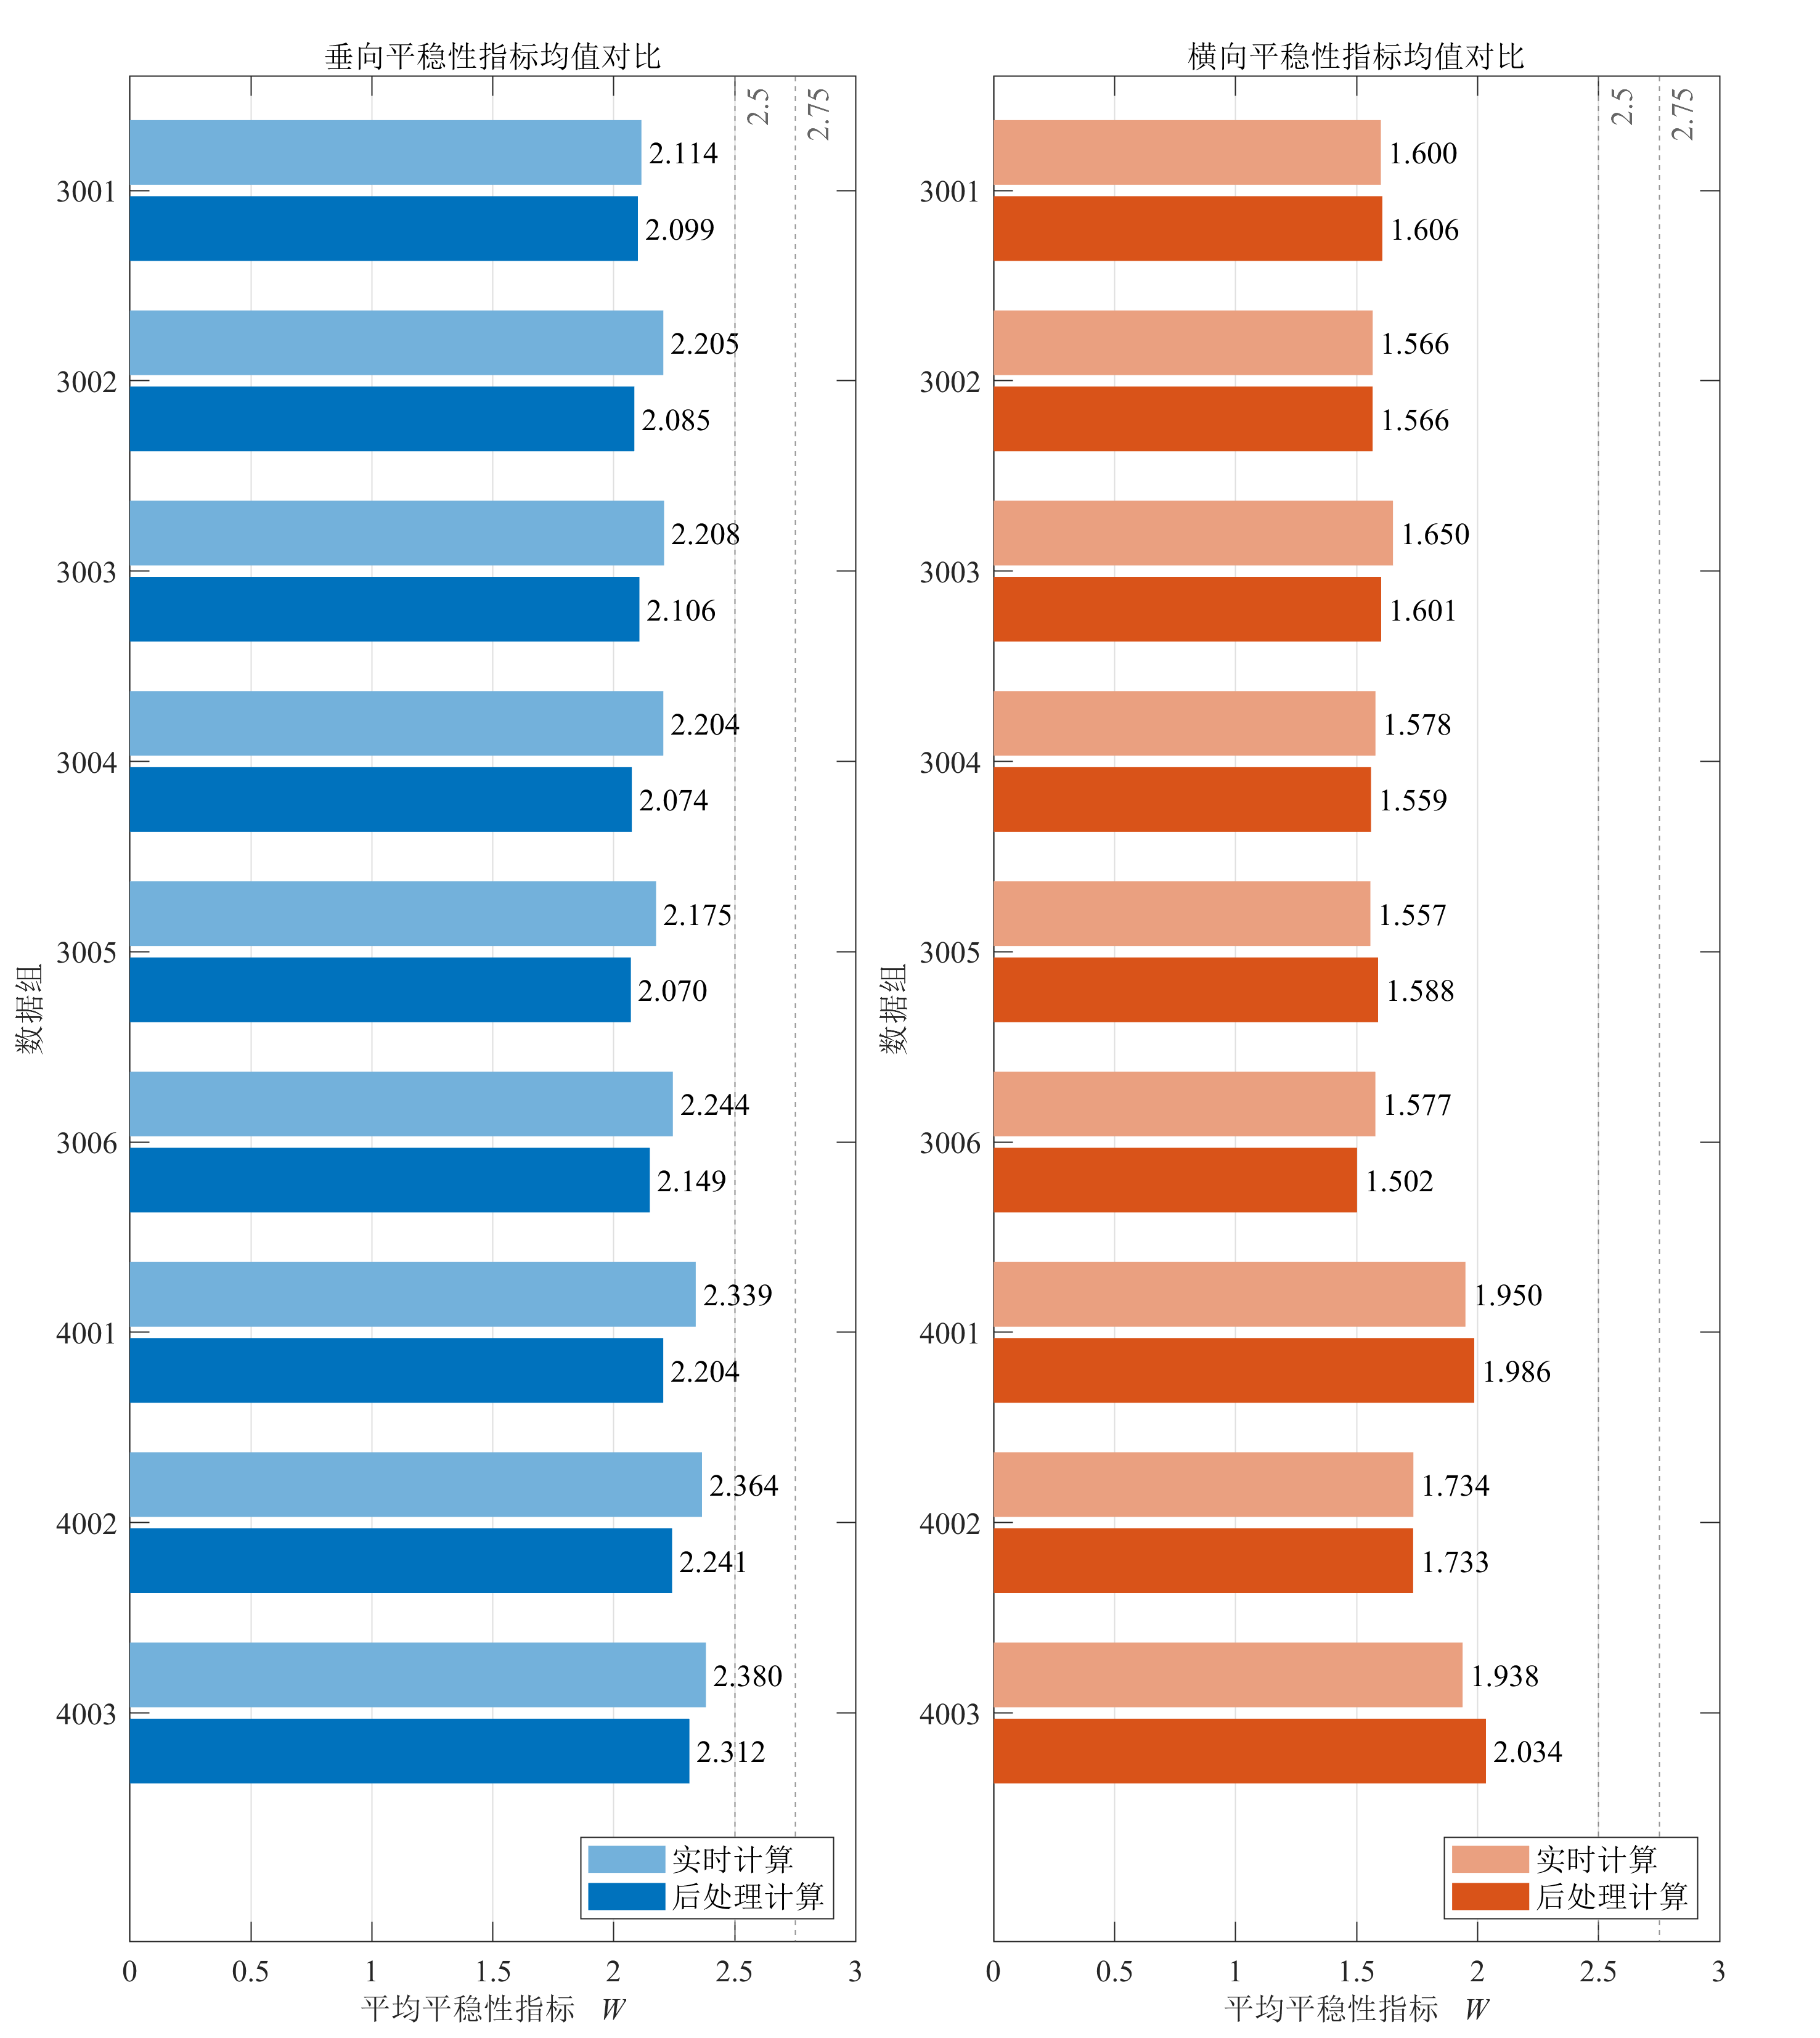
\includegraphics[width=0.98\linewidth]{pics/99_all_sperling_comparison.png}
    \vspace{-0.1cm}
    \caption{实时计算与后处理计算的平稳性指标均值对比}
    \label{fig:sperling-comparison}
    \vspace{-0.5cm}
\end{figure}

\subsection{\heiti{实验结论}}
\par{}
由图\ref{fig:sperling-comparison}可见，两种方法得到的所有平稳性指标均值都小于2.5，即在实验条件下，长时间运行的列车运行平稳性均值可以达到优级。但实时计算结果中，4002组和4003组垂向的$W_3$分别为2.56042和2.53259，均超过2.5。因此，个别时段的平稳性仍有所下降。
\par{}
本次测试中，各组垂向平稳性指标均值均大于对应的横向均值；40~km/h时的指标均值总体高于30~km/h。这表明本次测试条件下，垂向平稳性相对较差，较高速度工况下的平稳性也相对低速较差。
\par{}
此外发现垂向的实时计算结果都略大于对应的后处理计算结果，但是横向的并不明显，这可能与实时程序和后处理程序的频带处理方式不同，以及数据分段区间及预处理设置的不同有关。这些差异在误差允许范围内都是可接受的，因此也证明了实验条件下，采用类似方法得到的后处理结果和实时计算结果能够相互印证。

\subsection{\heiti{现场照片与程序源代码}}
\par{}
实验现场照片见图\ref{fig:test-line}至图\ref{fig:onboard-test}，MATLAB后处理脚本源代码见文末。

\begin{figure}[H]
    \centering
    \begin{minipage}[t]{0.48\linewidth}
        \centering
        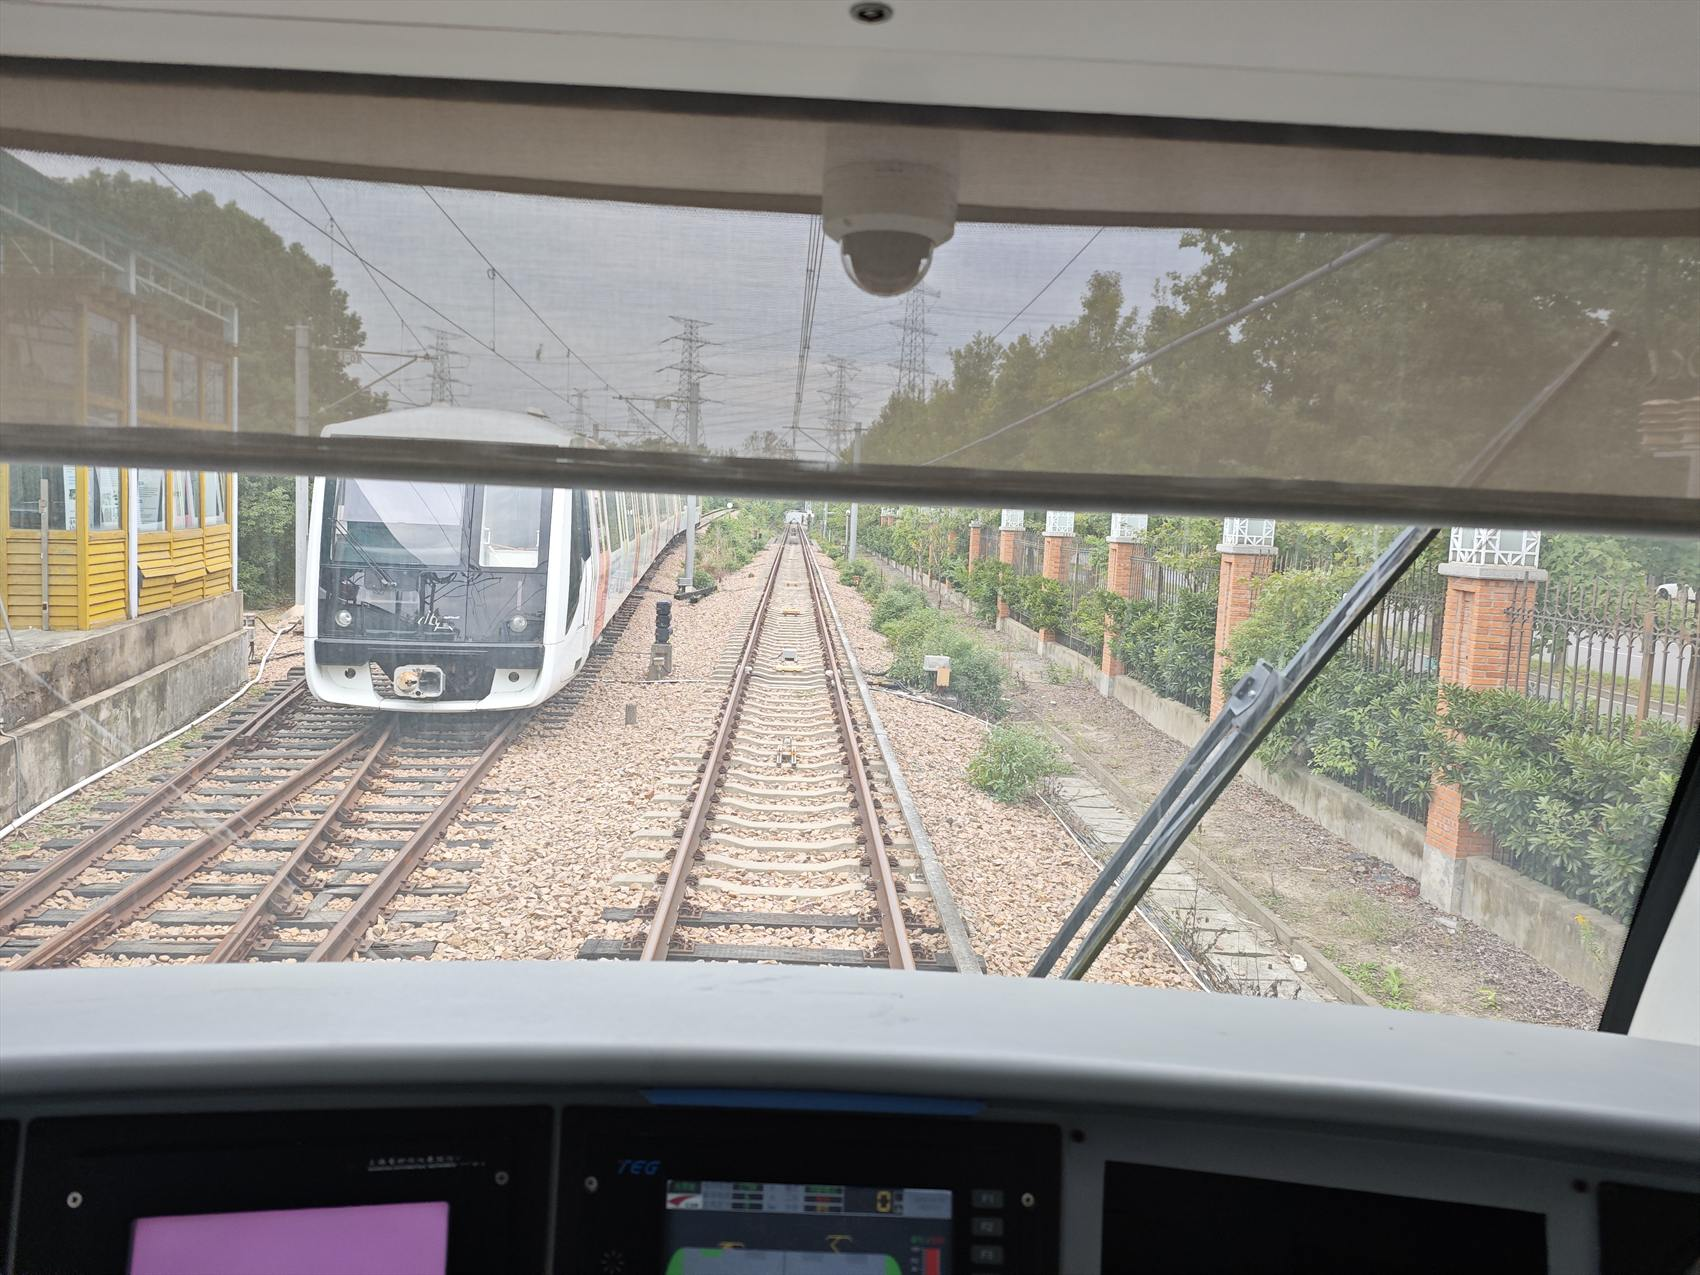
\includegraphics[width=\linewidth]{pics/06.jpg}
        \caption{驾驶室视角}
        \label{fig:test-line}
    \end{minipage}\hfill
    \begin{minipage}[t]{0.48\linewidth}
        \centering
        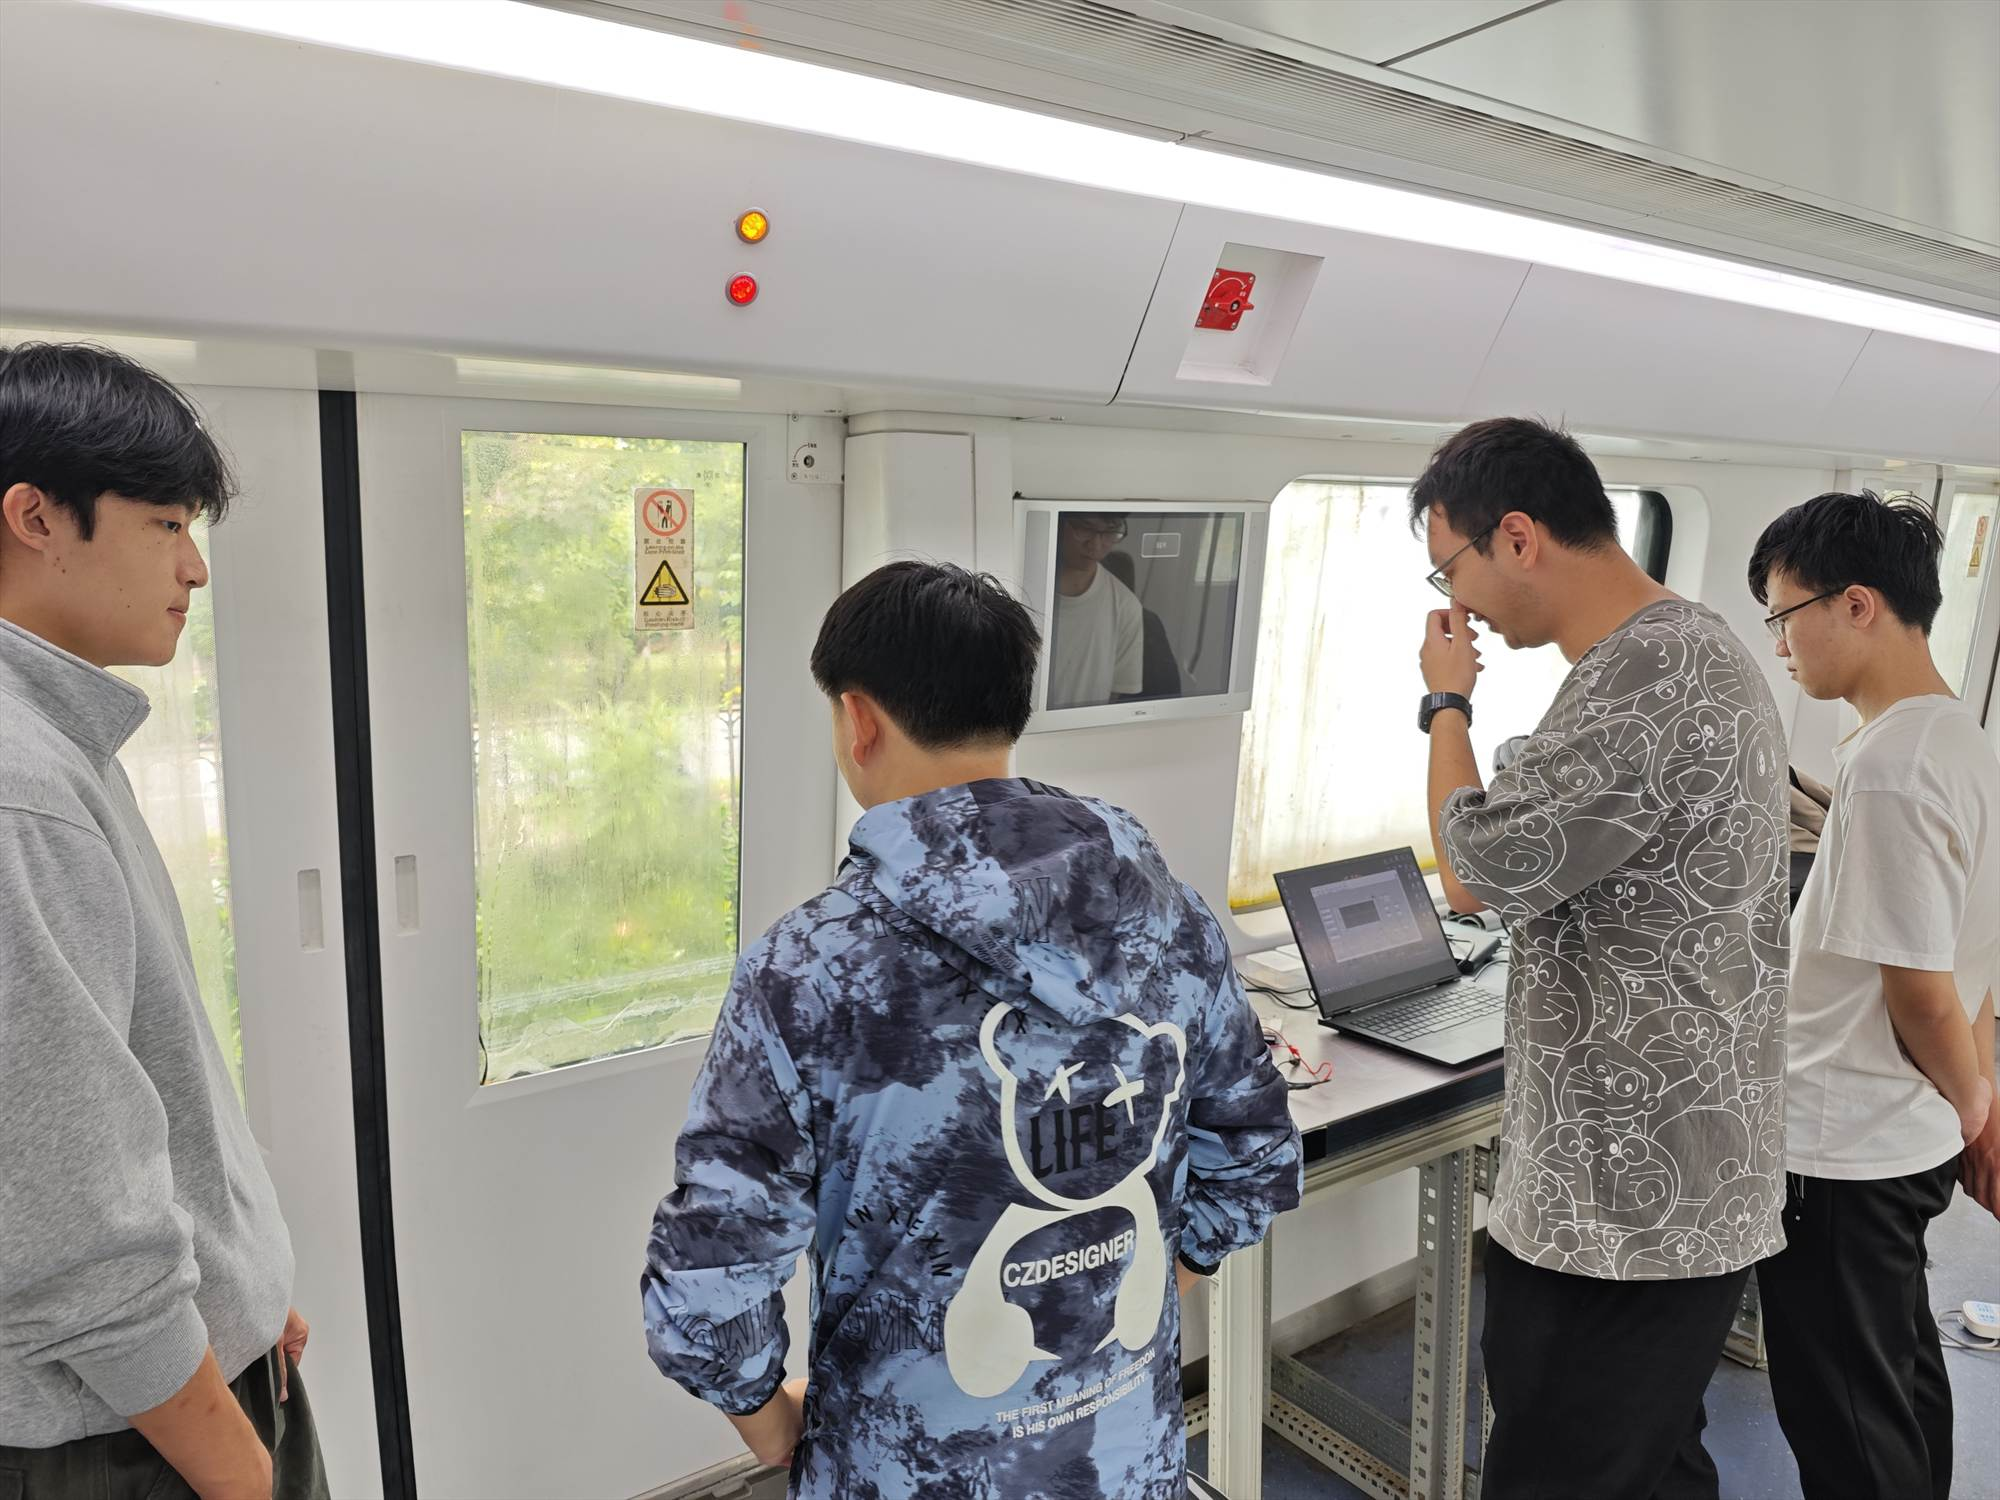
\includegraphics[width=\linewidth]{pics/07.jpg}
        \caption{车载数据采集现场}
        \label{fig:onboard-acquisition}
    \end{minipage}
\end{figure}

\begin{figure}[H]
    \centering
    \begin{minipage}[t]{0.48\linewidth}
        \centering
        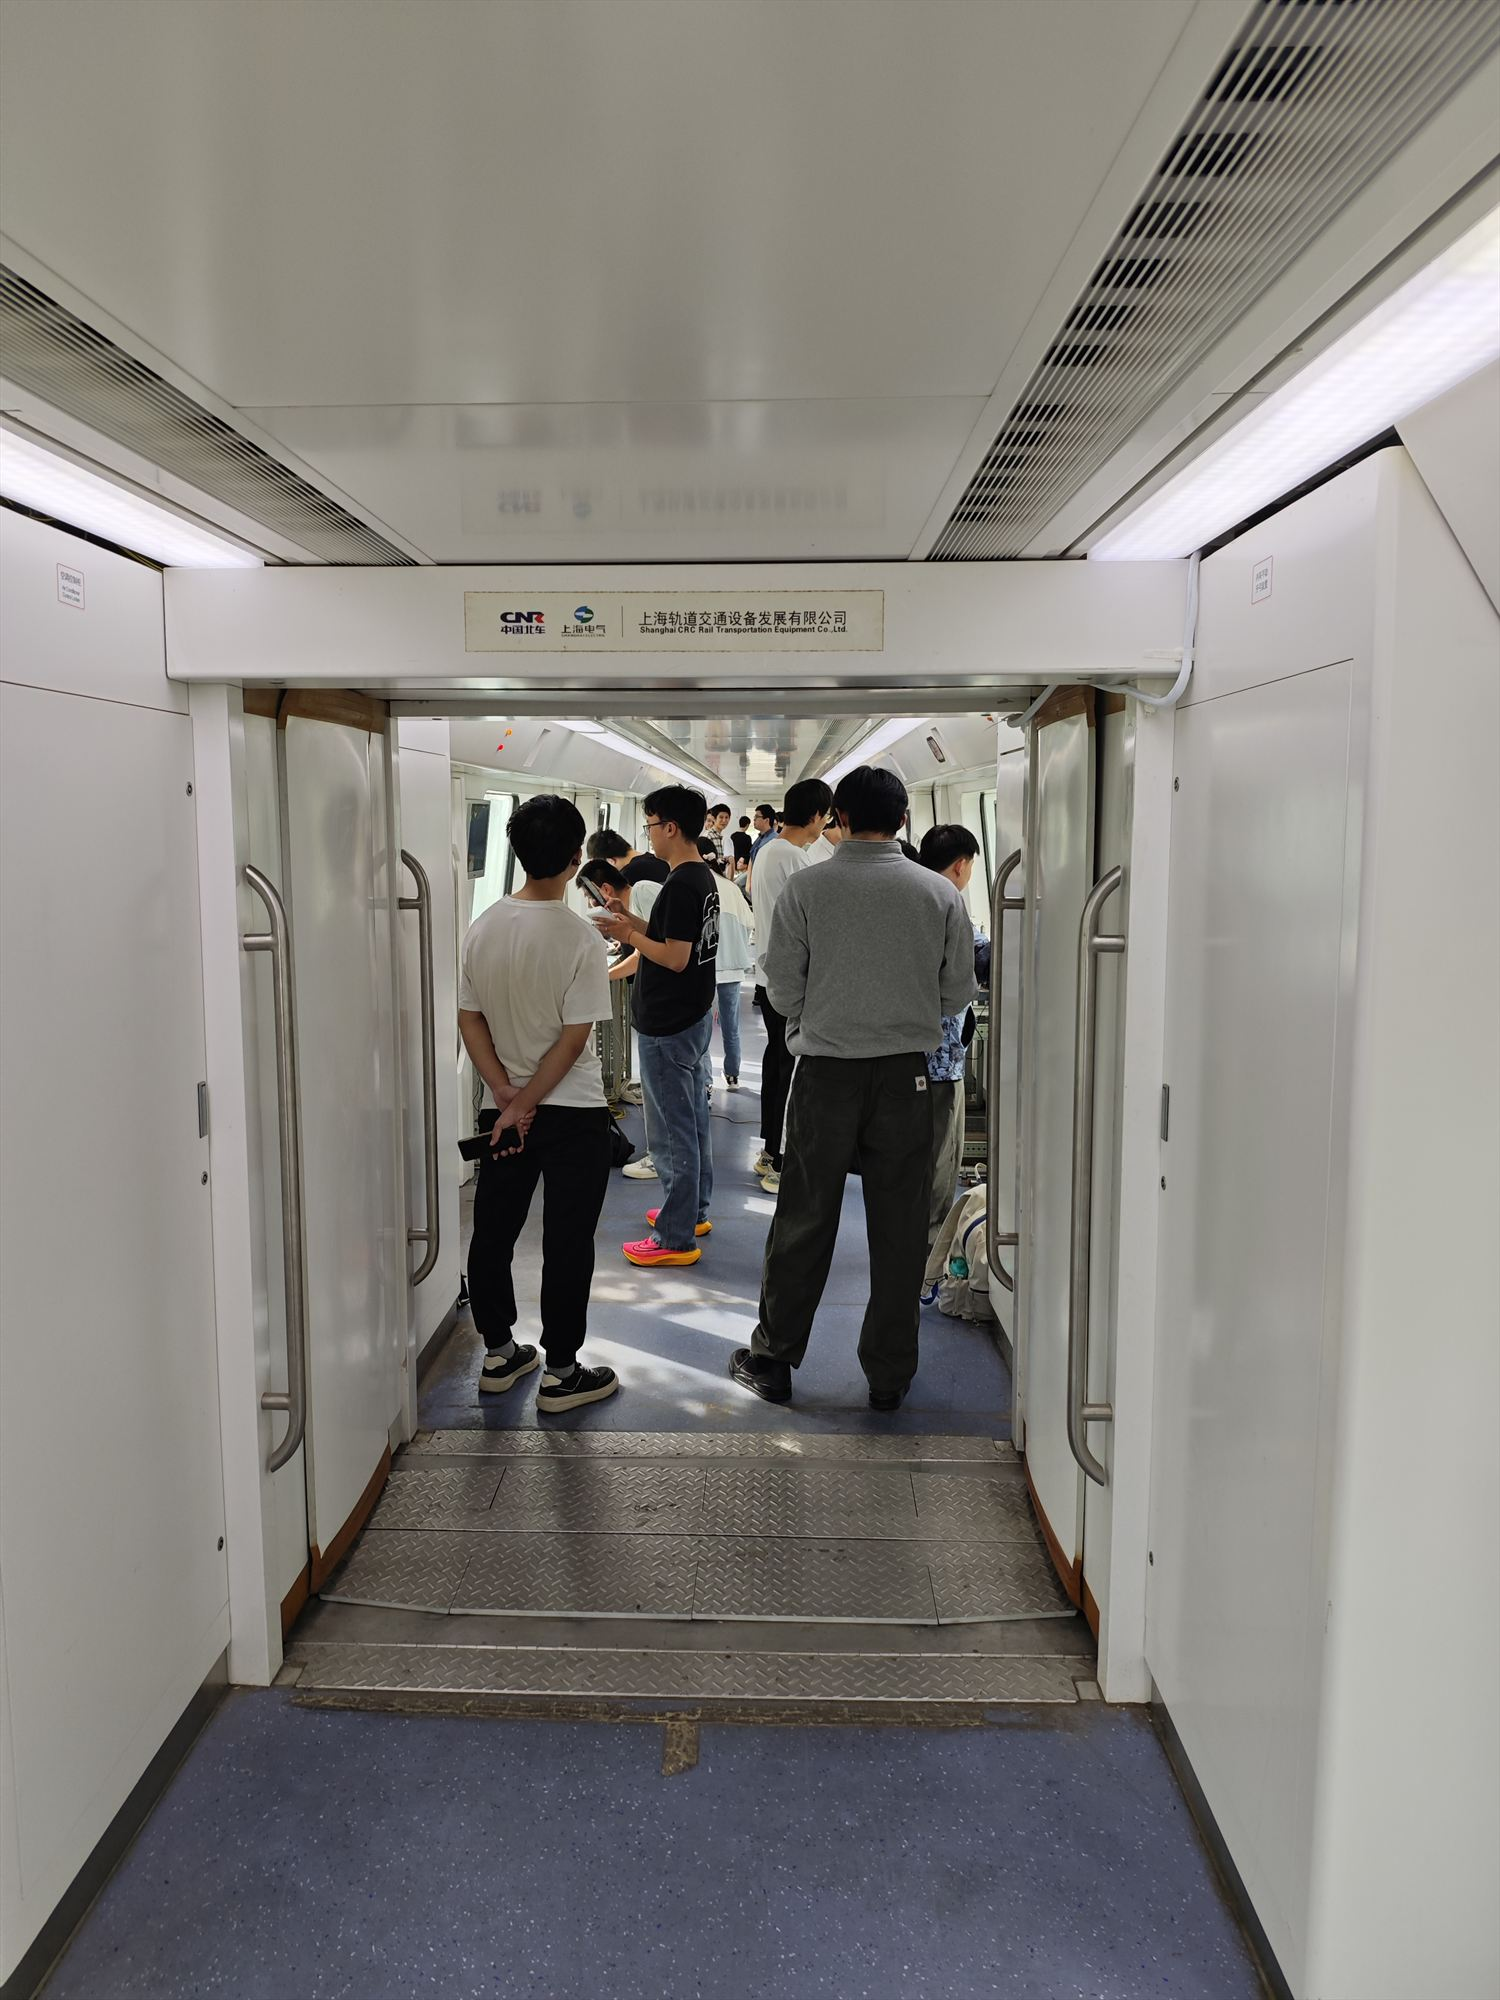
\includegraphics[width=\linewidth]{pics/08.jpg}
        \caption{车内测试现场}
        \label{fig:test-car-interior}
    \end{minipage}\hfill
    \begin{minipage}[t]{0.48\linewidth}
        \centering
        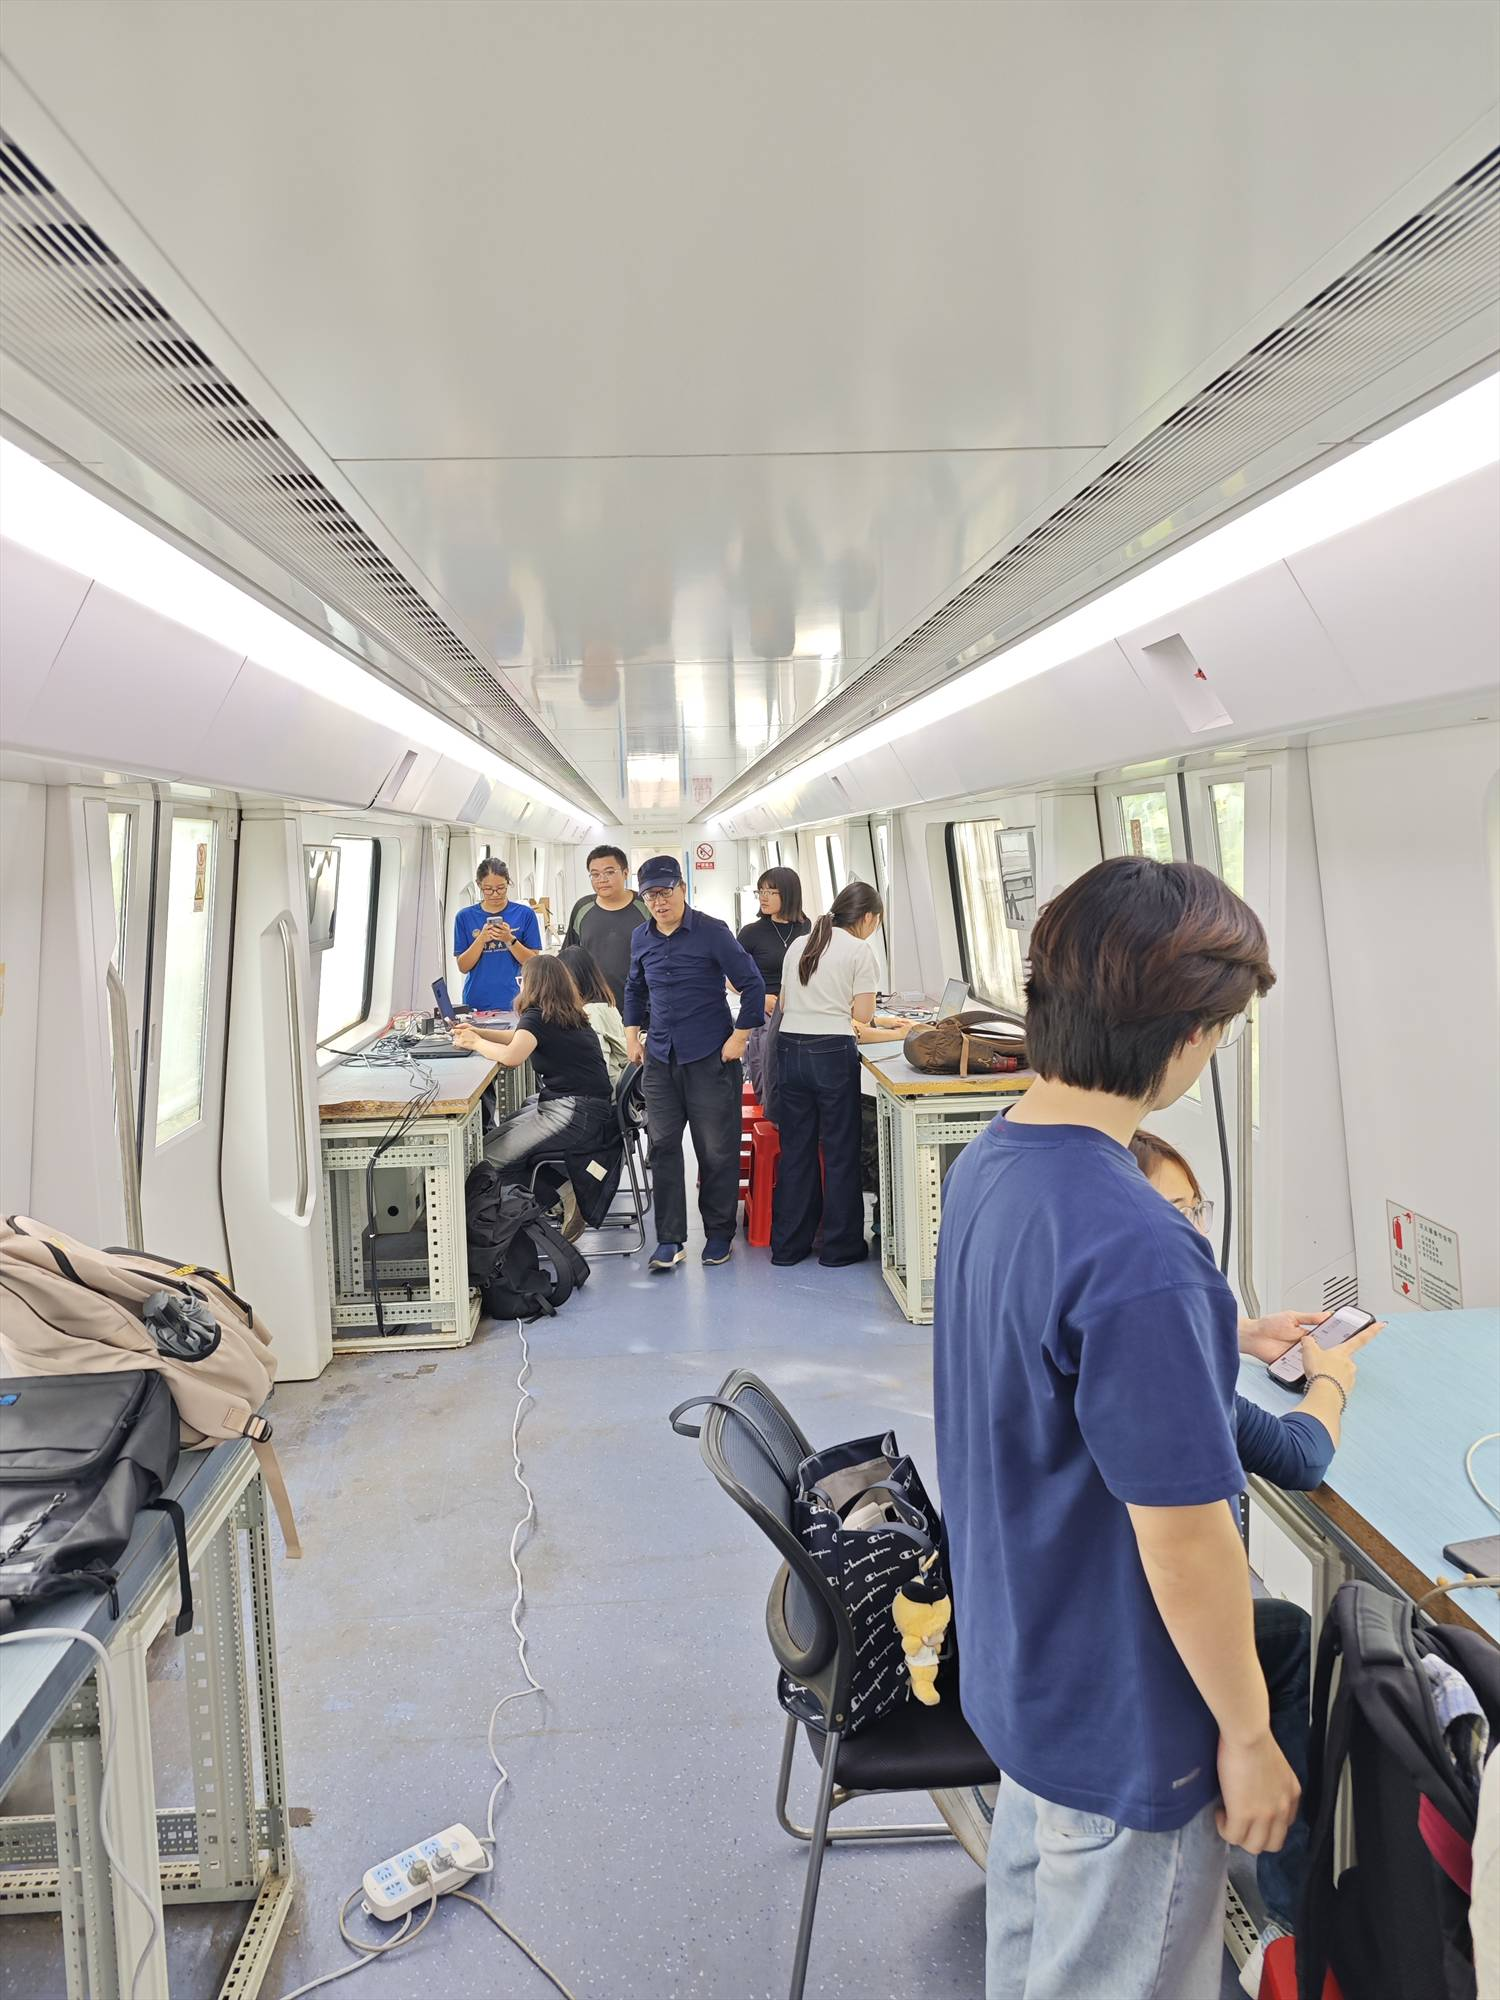
\includegraphics[width=\linewidth]{pics/09.jpg}
        \caption{车内测试现场}
        \label{fig:onboard-test}
    \end{minipage}
\end{figure}

\par{}
\newgeometry{left=0pt,right=0pt,top=0pt,bottom=0pt}
\thispagestyle{empty}
\begin{figure}[htbp]
    \centering
    \special{papersize=\the\paperwidth, 1551.97mm}
    
\includegraphics[width=\paperwidth]{pics/10.png}
\end{figure}

\end{document}
